\section{Part 2: Creating your own target}

\begin{frame}{Part 2}

Creating your own target

\end{frame}

%%%%%%%%%%%%%%%%%%%%%%%%%%%%%%%%%%%%%%%%%%%%%%%%%%%%%%%%%%%%%%%%%%%%%%%%%%%%%%%%

\begin{frame}{Bits of your ISA you need to describe}

\begin{itemize}
    \item Target machine
    \begin{itemize}
        \item Registers, register classes
        \item Calling conventions
    \end{itemize}
    \item Instruction set
    \begin{itemize}
        \item Operands and patterns
        \item Assembly printing and/or instruction encoding
        \item Schedule (not part of this talk)
    \end{itemize}
    \item ...
\end{itemize}

\end{frame}

%%%%%%%%%%%%%%%%%%%%%%%%%%%%%%%%%%%%%%%%%%%%%%%%%%%%%%%%%%%%%%%%%%%%%%%%%%%%%%%%

\begin{frame}{TableGen}

\begin{itemize}
    \item C++-style syntax
    \item Different set of backends
    \begin{itemize}
        \item RegisterInfo, InstrInfo, AsmWriter, ...
    \end{itemize}
    \item TableGen backends generate .inc files
    \begin{itemize}
        \item Included by your C++ files
    \end{itemize}
    \item More information:
    \begin{itemize}
        \item \url{llvm.org/docs/TableGen/index.html}
        \item \url{llvm.org/docs/TableGen/BackEnds.html}
    \end{itemize}
\end{itemize}

\end{frame}

%%%%%%%%%%%%%%%%%%%%%%%%%%%%%%%%%%%%%%%%%%%%%%%%%%%%%%%%%%%%%%%%%%%%%%%%%%%%%%%%

\begin{frame}[fragile]{Describing registers with TableGen}

\begin{itemize}
    \item TableGen provides the 'Register' class
    \begin{itemize}
        \item Can use the 'HWEncoding' field for encodings
    \end{itemize}
    \item Referenced as “LEG::R0” in C++
\end{itemize}

\begin{block}{LEGRegisterInfo.td}
\begin{lstlisting}
class LEGReg<bits<16> Enc, string n> : Register<n> {
  Let HWEncoding = Enc;
  let Namespace = "LEG";
}

def R0 : LEGReg< 0, "r0" >;
...
def SP : LEGReg< 10, "sp" >;
\end{lstlisting}
\end{block}

\end{frame}

%%%%%%%%%%%%%%%%%%%%%%%%%%%%%%%%%%%%%%%%%%%%%%%%%%%%%%%%%%%%%%%%%%%%%%%%%%%%%%%%

\begin{frame}[fragile]{Describing registers with TableGen}

\begin{itemize}
    \item Can automate trivial definitions
\end{itemize}

\begin{block}{LEGRegisterInfo.td}
\begin{lstlisting}
foreach i = 0-9 in {
  def R#i : R<i, "r"#i>;
}
\end{lstlisting}
\end{block}

\begin{itemize}
    \item Group registers into register classes
\end{itemize}

\begin{block}{LEGRegisterInfo.td}
\begin{lstlisting}
def GRRegs : RegisterClass<"LEG", [i32], 32,
  (add SP, (sequence "R%i", 0, 9))>;
\end{lstlisting}
\end{block}

\end{frame}

%%%%%%%%%%%%%%%%%%%%%%%%%%%%%%%%%%%%%%%%%%%%%%%%%%%%%%%%%%%%%%%%%%%%%%%%%%%%%%%%

\begin{frame}[fragile]{Calling convention lowering: TableGen}

\begin{block}{LEGCallingConv.td}
\begin{lstlisting}
def CC_LEG : CallingConv<[
    // Promote i8/i16 arguments to i32
    CCIfType<[i8, i16], CCPromoteToType<i32>>,

    // The first 4 arguments are passed in registers
    CCIfType<[i32], CCAssignToReg<[R0, R1, R2, R3]>>,

    // Fall-back, and use the stack
    CCIfType<[i32], CCAssignToStack<4, 4>>
  ]>;
\end{lstlisting}
\end{block}

\begin{itemize}
    \item Generates functions used in ISelLowering via function pointers.
\end{itemize}

\end{frame}

%%%%%%%%%%%%%%%%%%%%%%%%%%%%%%%%%%%%%%%%%%%%%%%%%%%%%%%%%%%%%%%%%%%%%%%%%%%%%%%%

\begin{frame}[fragile]{Calling convention lowering:
The big picture}

\begin{columns}[t]
\column{.5\textwidth}
    \begin{block}{ex1.ll}
    \begin{lstlisting}
define i32 @foo(i32 %a, i32 %b) {
    %c = add nsw i32 %a, %b
    ret i32 %c
}
    \end{lstlisting}
    \end{block}

    Two target hooks:
    \begin{itemize}
            \item LowerFormalArguments()
            \item LowerReturn()
    \end{itemize}
\column{.5\textwidth}
    % FIXME Add 'a', 'b', 'c' circles and color formatting of the .ll example
    \begin{block}{}
        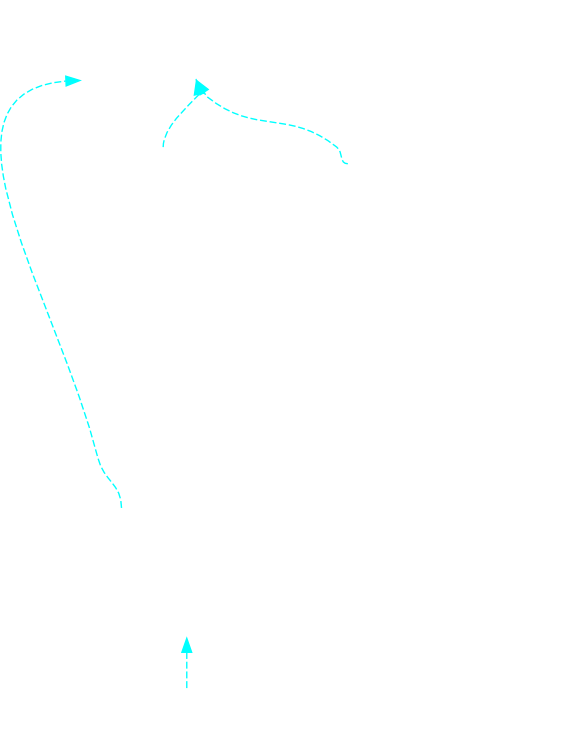
\includegraphics[width = 0.8\textwidth]{examples/ex1-entry-selection-dag.png}
    \end{block}
\end{columns}    

\end{frame}

%%%%%%%%%%%%%%%%%%%%%%%%%%%%%%%%%%%%%%%%%%%%%%%%%%%%%%%%%%%%%%%%%%%%%%%%%%%%%%%%

\begin{frame}[fragile]{Calling convention lowering: The big picture}

\begin{columns}[t]
\column{.5\textwidth}
    LowerFormalArguments()
    \begin{itemize}
        \item Lowers incoming arguments into the DAG
    \end{itemize}

    LowerReturn()
    \begin{itemize}
        \item Lowers outgoing return values into the DAG
    \end{itemize}
    
\column{.5\textwidth}
    % FIXME Add 'a', 'b', 'c' circles and arrows from Lower*() to white circles
    \begin{block}{}
        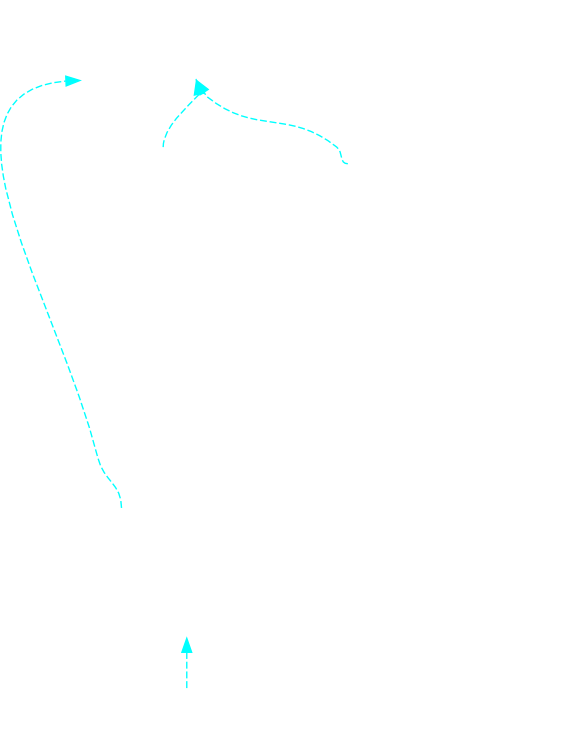
\includegraphics[width = 0.8\textwidth]{examples/ex1-entry-selection-dag.png}
    \end{block}
\end{columns}    

\end{frame}

%%%%%%%%%%%%%%%%%%%%%%%%%%%%%%%%%%%%%%%%%%%%%%%%%%%%%%%%%%%%%%%%%%%%%%%%%%%%%%%%

\begin{frame}[fragile]{Calling convention lowering: LowerFormalArguments()}

\begin{itemize}
    \item Assigns locations to arguments, according to the TableGen-defined calling convention
    \item Creates DAG nodes for each location:
    \begin{itemize}
        \item Registers: CopyFromReg nodes
        \item Stack: frame indices and stack loads
    \end{itemize}
\end{itemize}

\begin{block}{LEGISelLowering.cpp}
\begin{lstlisting}
// LEGTargetLowering::LowerFormalArguments()
SmallVector<CCValAssign, 16> ArgLocs;
CCState CCInfo(CallConv, isVarArg, DAG.getMachineFunction(),
               getTargetMachine(), ArgLocs,
               *DAG.getContext());
CCInfo.AnalyzeFormalArguments(Ins, CC_LEG);
...
\end{lstlisting}
\end{block}

\end{frame}

%%%%%%%%%%%%%%%%%%%%%%%%%%%%%%%%%%%%%%%%%%%%%%%%%%%%%%%%%%%%%%%%%%%%%%%%%%%%%%%%

\begin{frame}{Calling convention lowering: LowerReturn()}

\begin{itemize}
    \item Similar to LowerFormalArguments(), but the other way around
    \item Define another, 'RetCC\_LEG, TableGen calling convention
    \item Call 'AnalyzeReturn()' with it
    \item Walk the return value locations and issue DAG nodes
    \item Return LEGISD::RET instruction
\end{itemize}

\end{frame}

%%%%%%%%%%%%%%%%%%%%%%%%%%%%%%%%%%%%%%%%%%%%%%%%%%%%%%%%%%%%%%%%%%%%%%%%%%%%%%%%

\begin{frame}{Calling convention lowering: LowerCall()}

\begin{itemize}
    \item Hybrid of LowerFormalArguments() and LowerReturn()
    \item Not explicitly covered here
\end{itemize}

\end{frame}

